
\chapter{Optimization}

An \textit{optimization problem} has the form

\begin{equation}
    \begin{split}
        minimize &\;\;\;\;\; f_0(x) \\
        subject\;to &\;\;\;\;\; f_i(x) \leq b_i,\;\;\;\;\; i=1, \dots, m.
    \end{split}
\end{equation}


Here the vector $x=(x_1, \dots, x_n)$ is the optimization variable of the problem, the function $f_0~:~\mathbb{R}^n\rightarrow \mathbb{R}$ is the objective function, the functions $f_i~ :~\mathbb{R}^n\rightarrow~\mathbb{R}$, $i=1, \dots, m$, are the (inequality) constraint functions, and the constants $b_1, \dots, b_m$ are the limits, or bounds, for the constraints.

\section{Least-Squares}

A \textit{least-squares} problem is an optimization problem with no constraints and an objective function which is a sum of squares of terms of the form
\begin{equation}
    minimize \;\;\; f_0(x) = ||Ax-b||^2_2
\end{equation}

The solution of such a problem can be reduced to solving a set of linear equations

\begin{equation}
    (A^T A)x=A^Tb,
\end{equation}

which has the following analytical solution: $x = (A^TA)^{-1}A^Tb$.

Some variants exist:
\paragraph{Weighted least-squares} The cost becomes
\begin{equation}
    \sum_{i=1}^{k} w_i(a_i^Tx-b)^2
\end{equation}
which has the following solution: $x=(A^TWA)^{-1}A^TWb$.

\paragraph{Regularized least-squares} The cost is
\begin{equation}
    \sum_ {i=1}^k (a_i^Tx-b)^2 + \rho \sum_{i=1}^n x_i^2,
\end{equation}
Different type of regularizer (the second term) exist and are usually derived form a statistical point-of-view.

\section{Linear Programming}

Another important class of optimization problems is \textit{linear programming}, in which the objective and all constraint functions are linear:

\begin{equation}
    \begin{split}
        minimize &\;\;\;\;\; c^Tx \\
        subject\;to & \;\;\;\;\;a_i^Tx\leq b_i,\;\;\;i=1, \dots,m.
    \end{split}
\end{equation}

There is no analytical formula for the solution of a linear program (as there is for a least-squares problem), but there are a variety of very effective methods. The most famous one is probably the \textbf{simplex algorithm}.

\section{Convex optimization}

A convex optimization problem is one of the form

\begin{equation}
    \begin{split}
        minimize &\;\;\;\;\; f_0(x) \\
        subject\;to &\;\;\;\;\; f_i(x) \leq b_i,\;\;\;\;\; i=1, \dots, m.
    \end{split}
\end{equation}

where the functions $f_0, \dots,f_m : \mathcal{R}^n\rightarrow\mathcal{R}$ are convex, \textit{i.e.}, satisfy
\begin{equation}
    f_i(\alpha x+\beta y)\leq \alpha f_i(x)+\beta f_i(y)
\end{equation}
for all $x,y\in\mathcal{R}^n$ and all $\alpha, \beta \in \mathcal{R}$ with $\alpha+\beta=1$, $\alpha\geq0, \beta\geq0$.

The least-squares problem and the linear programming problem are both special cases of the general convex optimization problem (as convex is a bit more general than linear).

\section{Non-linear optimization}


\subsection{Convexity}


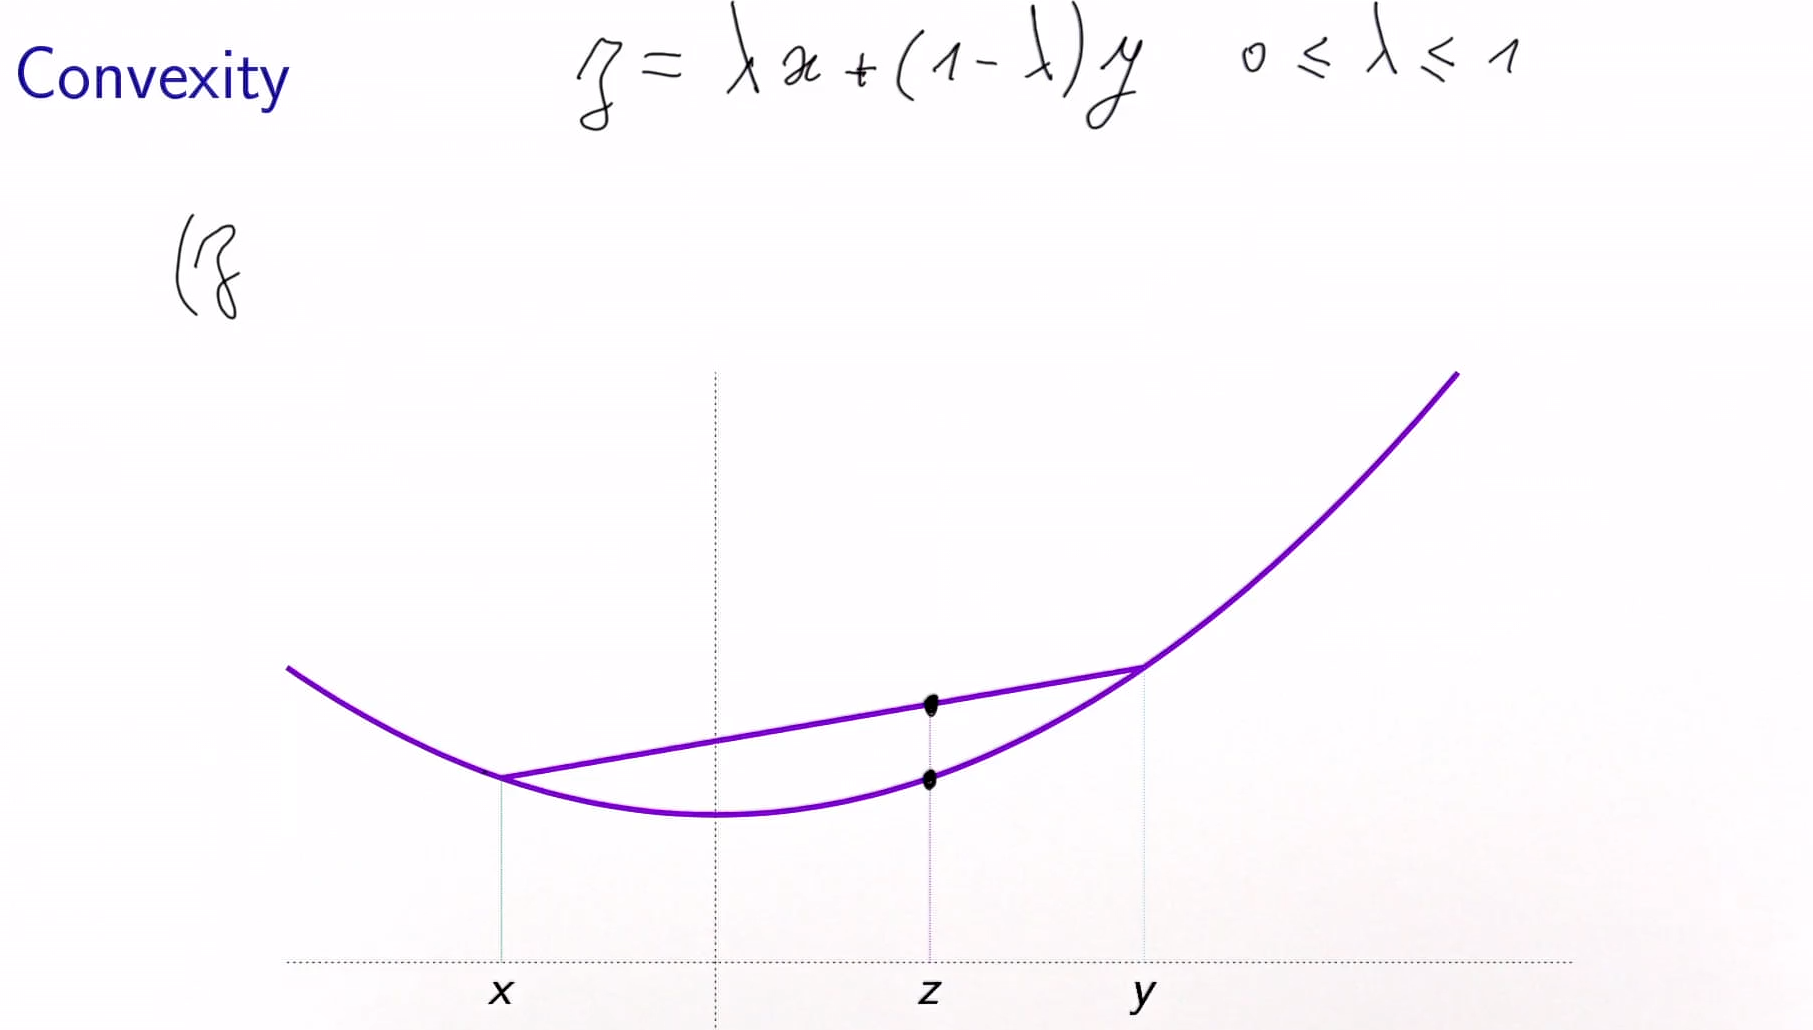
\includegraphics[width=\linewidth]{content/convexity.png}

If the objective function of an optimization problem is convex, it is possible to find a global optimum.

\subsection{First derivative}
The gradient of a function is defined as:

\begin{equation}
    \nabla f(x)=\left(\begin{array}{c}
        \frac{\delta f(x)}{\delta x_1} \\
        \vdots \\
        \frac{\delta f(x)}{\delta x_n}
    \end{array}\right)
\end{equation}

$d$ is a descent direction if $d^T\nabla f(x) < 0$.

For several functions, $f: \mathbb{R}^n\rightarrow\mathbb{R}^m$, the \textbf{Jacobian} matrix is defined as:
\begin{equation}
    J(x) = \left(\begin{array}{c}
        \nabla f_1(x)^T \\
        \vdots  \\
        \nabla f_m(x)^T \\
    \end{array}\right) = \left(\begin{array}{ccc}
        \frac{\delta f_0(x)}{\delta x_0} & \dots & \frac{\delta f_0(x)}{\delta x_n} \\
         \vdots & \ddots & \vdots \\
        \frac{\delta f_m(x)}{\delta x_0} & \dots & \frac{\delta f_m(x)}{\delta x_n} \\
    \end{array}\right)
\end{equation}

The first derivate of a functions describe its slope.



\subsection{Second derivatives}
\begin{equation}
    \nabla f(x): \mathbb{R}^n\rightarrow\mathbb{R}^n
\end{equation}

The gradient matrix of $\nabla f(x)$ is called the \textbf{Hessian} or the second derivatives matrix when it exists:

\begin{equation}
    \nabla(\nabla(f(x))=\nabla^2f(x) \;\; \in \mathbb{R}^n
\end{equation}
The Hessian matrix is symmetric.

If $\nabla^2 f(x)$ is positive semidefinite on $X\subseteq\mathbb{R}^n$, then $f$ is convex on $X$.


The second derivatives of a function give information about the curvature of the function. The curvature of $f$ in $x$ in direction $d$ is defined as
\begin{equation}
    \frac{d^T\nabla^2 f(x)d}{d^Td}
\end{equation}

\subsection{Linearity and nonlinearity}

A function is linear if it is a linear combination of the parameters:
\begin{equation}
\begin{split}
    f: \mathbb{R}^n \rightarrow \mathbb{R}:&\;\;\; f(x) = \sum_{i=1}^n c_i x_i = c^T x \;\;\; c\in\mathbb{R}^n \\
    f: \mathbb{R}^n \rightarrow \mathbb{R}^m:&\;\;\; f(x) = Ax \;\;\; A\in\mathbb{R}^{m\times n}
\end{split}
\end{equation}

Affine functions are very close
\begin{equation}
\begin{split}
    f(x) = c^T+d \\
    f(x) = Ax+b
\end{split}
\end{equation}

They are usually also included in the term "linear" because the additional constant does not play any role in the optimization.


However, most functions encountered in reality are nonlinear. Actually, a function can have different level of nonlinearity.

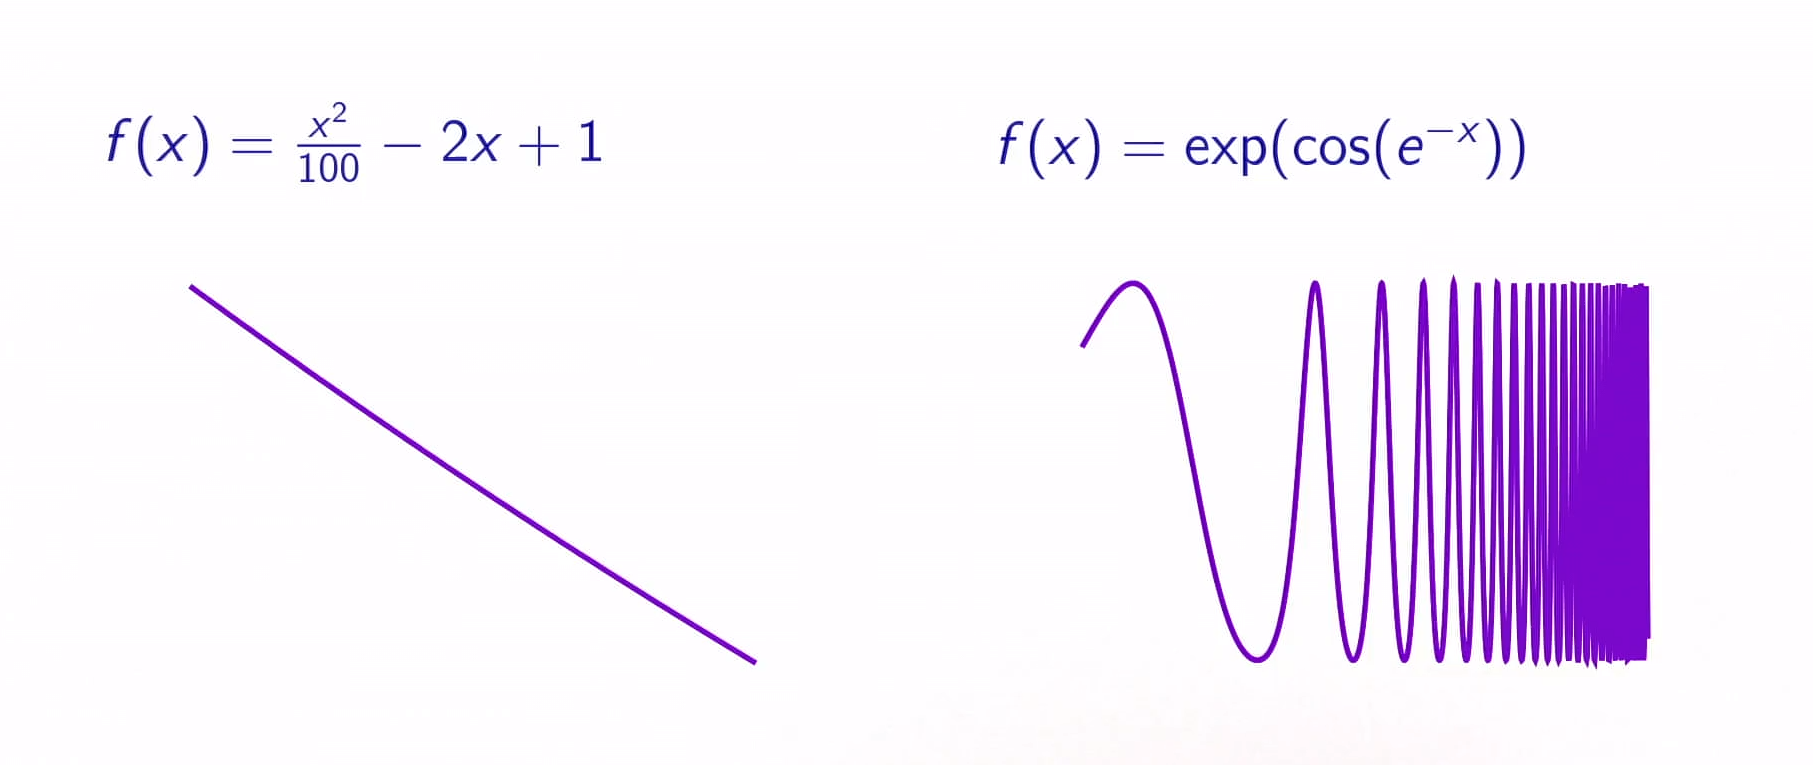
\includegraphics[width=\linewidth]{content/nonlinearity.png}

To characterize if a function is linear or not, we analyze how quickly its derivative is changing. 
The gradient of $f$ is Lipschitz continuous if there exist a $M > 0$ such that, for all $x, y$:
\begin{equation}
    ||\nabla f(x)-\nabla f(y)|| \leq M||x-y||
\end{equation}
M is called the \textbf{Lipschitz constant} of the function.
\begin{itemize}
    \item a small value correspond to almost linear functions
    \item a large value correspond to highly nonlinear functions
\end{itemize}

\subsection{Preconditioning}

The \textbf{condition number} is an indicator of the geometry of a function and its value influences a lot some of the algorithms.
It is possible to change the formulation of the problem in order to get a better value for this indicator. This modification is called \textit{preconditioning}.

\begin{equation}
    k(A) = ||A||\cdot||A^{-1}]||
\end{equation}

and if the matrix $A$ is symmetric positive semidefinite, the condition number is the ratio between the largest and smallest eigen values: $k(A) = \frac{\lambda_1}{\lambda_n}$.


For a function with $\nabla^2 f(x)$ positive definite, the eigen value $\lambda_1$ corresponds to the curvature of the function in the direction of its corresponding eigen vector $d_1$. This means that the conditioning number is the ratio between the largest and the smallest curvature.

For example, a 2D function like a valley has a very high curvature in one direction and a small curvature in the orthogonal direction. This means that its condition number is very high, which causes problem during optimization (called ill-conditioned).

The condition number of a function can be modified by a change of variables. Let $M$ be an invertible matrix that defines this change of variable: $x^{\prime}=Mx$ and $x=M^{-1}x^{\prime}$

\begin{equation}
    \begin{split}
        \tilde{f}(x^{\prime}) & = f(M^{-1}x^{\prime}) \\
        \nabla\tilde{f}(x^{\prime}) & = M^{-T}\nabla f(M^{-1}x^{\prime}) \\
        \nabla^2\tilde{f}(x^{\prime}) & = M^{-T}\nabla^2 f(M^{-1}x^{\prime})M^{-1} \\
        & = M^{-T}\nabla^2 f(x)M^{-1}
    \end{split}
\end{equation}